\documentclass[11pt]{article}
\usepackage{amsmath}
\usepackage{graphicx}
\usepackage{hyperref}
\usepackage{enumitem}
\usepackage{geometry}
\geometry{a4paper, margin=0.75in}

\title{Data-Driven Agricultural Decision Making: Anomaly Detection, Analytics, and Simulation in Cattle Farms}
\author{Kevin George}
\date{\today}

\begin{document}

\begin{titlepage}
    \centering
    \vspace*{0.3in}
    \LARGE\textbf{Data-Driven Agricultural Decision Making: A Platform for Anomaly Detection, Analytic Reporting, and Simulation}\par
    \vspace{0.5in}
    \large Kevin George\par
    \vspace{0.2in}
    \normalsize \today
    \thispagestyle{empty}
\end{titlepage}

\section*{1. Motivation}
Advancing smart agriculture through the use of real sensor data is crucial for improving farm management, animal welfare, and resource optimization. By focusing on cattle farms, this research aims to leverage sensor data to enhance operations, ensure animal welfare, and manage resources more effectively, facilitating smarter decision-making.

\section*{2. Problem Definition}
\begin{itemize}
    \item \textbf{Data Management Platform:} Collecting sensor data and storing it in a university database.
    \item \textbf{Analytic Reporting:} Create tools to derive insights from sensor data.
    \item \textbf{Pattern Recognition and Anomaly Detection:} Improve methods for recognizing patterns and detecting anomalies in cattle behavior and sensor functionality.
    \item \textbf{Utilization of Simulated Data:} Enhance simulation accuracy with real ground truth data for better evaluation and validation of patterns and anomalies.
    \item \textbf{Semantic Models:} Utilize semantic models to improve data integration, quality, and interpretation.
\end{itemize}

\section*{3. Related Fields}
\begin{itemize}
    \item \textbf{Precision Agriculture:} Techniques and technologies aimed at monitoring and managing field variability in crops and livestock.
    \item \textbf{Internet of Things (IoT):} Deployment of interconnected sensors and devices in agricultural settings for real-time data collection and analysis.
    \item \textbf{Big Data Analytics:} Leveraging large datasets to extract meaningful insights, trends, and patterns in agricultural contexts.
    \item \textbf{Machine Learning:} Applications of machine learning algorithms for predictive modeling, anomaly detection, and decision support in agriculture.
    \item \textbf{Semantic Web and Ontologies:} Use of semantic models to integrate and interpret diverse data sources, enhancing data interoperability and contextual understanding.
\end{itemize}

\section*{4. Related Work}
\begin{itemize}
    \item \textbf{SmartSPEC Framework:} Chio, A., et al.
    \item \textbf{Beacon-Based Agricultural Data Simulation:} Paul Pongratz
    \item \textbf{Extending the Farm Simulator for Outdoor Data:} David Jares
    \item \textbf{Big Data Analytics for Smart Farming:} Sundararajan, S. S., et al.
    \item \textbf{Machine Learning for Anomaly Detection in Agriculture:} Alimi, A. M., et al.
    \item \textbf{Semantic Models in Agriculture:} Smith, J., et al.
\end{itemize}

\section*{5. Approach}
\begin{enumerate}[label=\arabic*., wide=0pt, left=0pt]
    \item \textbf{Data Collection:} Gather real sensor data from cattle farms.
    \item \textbf{Centralized Data Platform:} Implement a university-based platform for data collection, storage, processing, retrieval, and reporting.
    \item \textbf{Analytic Reporting Tools:} Develop tools to extract actionable insights from sensor data.
    \item \textbf{Pattern Recognition and Anomaly Detection:} Refine methods for identifying patterns and anomalies in cattle behavior and sensor functionality. Use semantic models to enhance accuracy and context.
    \item \textbf{Integration and Enhancement:} Integrate real sensor data into SmartSPEC and improve the farm simulator for more accurate simulations.
\end{enumerate}

\section*{6. Evaluation}
\textbf{Experiments:} Use real sensor data from cattle farms and simulated data generated using SmartSPEC to evaluate:
\begin{itemize}
    \item \textbf{Pattern and Anomaly Detection:} Assess the effectiveness of methods in detecting patterns and anomalies in both real and simulated data, utilizing semantic models to enhance interpretation.
    \item \textbf{Analytic Reporting:} Evaluate the efficacy of analytic tools in deriving actionable insights from real and simulated data.
    \item \textbf{Comparison with Related Work:} Compare performance against existing solutions using both real and simulated data.
    \item \textbf{Expected Results:} Achieve enhanced data quality and better decision-making supported by both real-world and simulated data.
\end{itemize}

\section*{7. Project Plan}
\begin{itemize}
    \item \textbf{July:} Conduct literature review and begin initial data collection.
    \item \textbf{August:} Implement centralized database platform for data management.
    \item \textbf{September:} Develop methods for pattern recognition, create behavior graphs, and detect anomalies.
    \item \textbf{October:} Develop and refine analytic tools, and enhance pattern recognition and anomaly detection methods with semantic models.
    \item \textbf{November:} Integrate real data with SmartSPEC, enhance the simulator, conduct experiments, and evaluate results.
    \item \textbf{December:} Finalize thesis and prepare for defense.
\end{itemize}

\section*{References}
\begin{itemize}
    \item Chio, A., et al. "SmartSPEC: Customizable Smart Space Datasets via Event-driven Simulations."
    \item Pongratz, P. "Beacon Data Simulation in Agriculture."
    \item Jares, D. "Extending the Farm Simulator for Outdoor Data."
    \item Sundararajan, S. S., et al. "Big Data Analytics for Smart Farming."
    \item Alimi, A. M., et al. "Machine Learning for Anomaly Detection in Agriculture."
    \item Smith, J., et al. "Semantic Models in Agriculture: Enhancing Data Integration and Quality."
\end{itemize}


\section*{Additional Explanation}

\begin{figure}[h!]
    \centering
    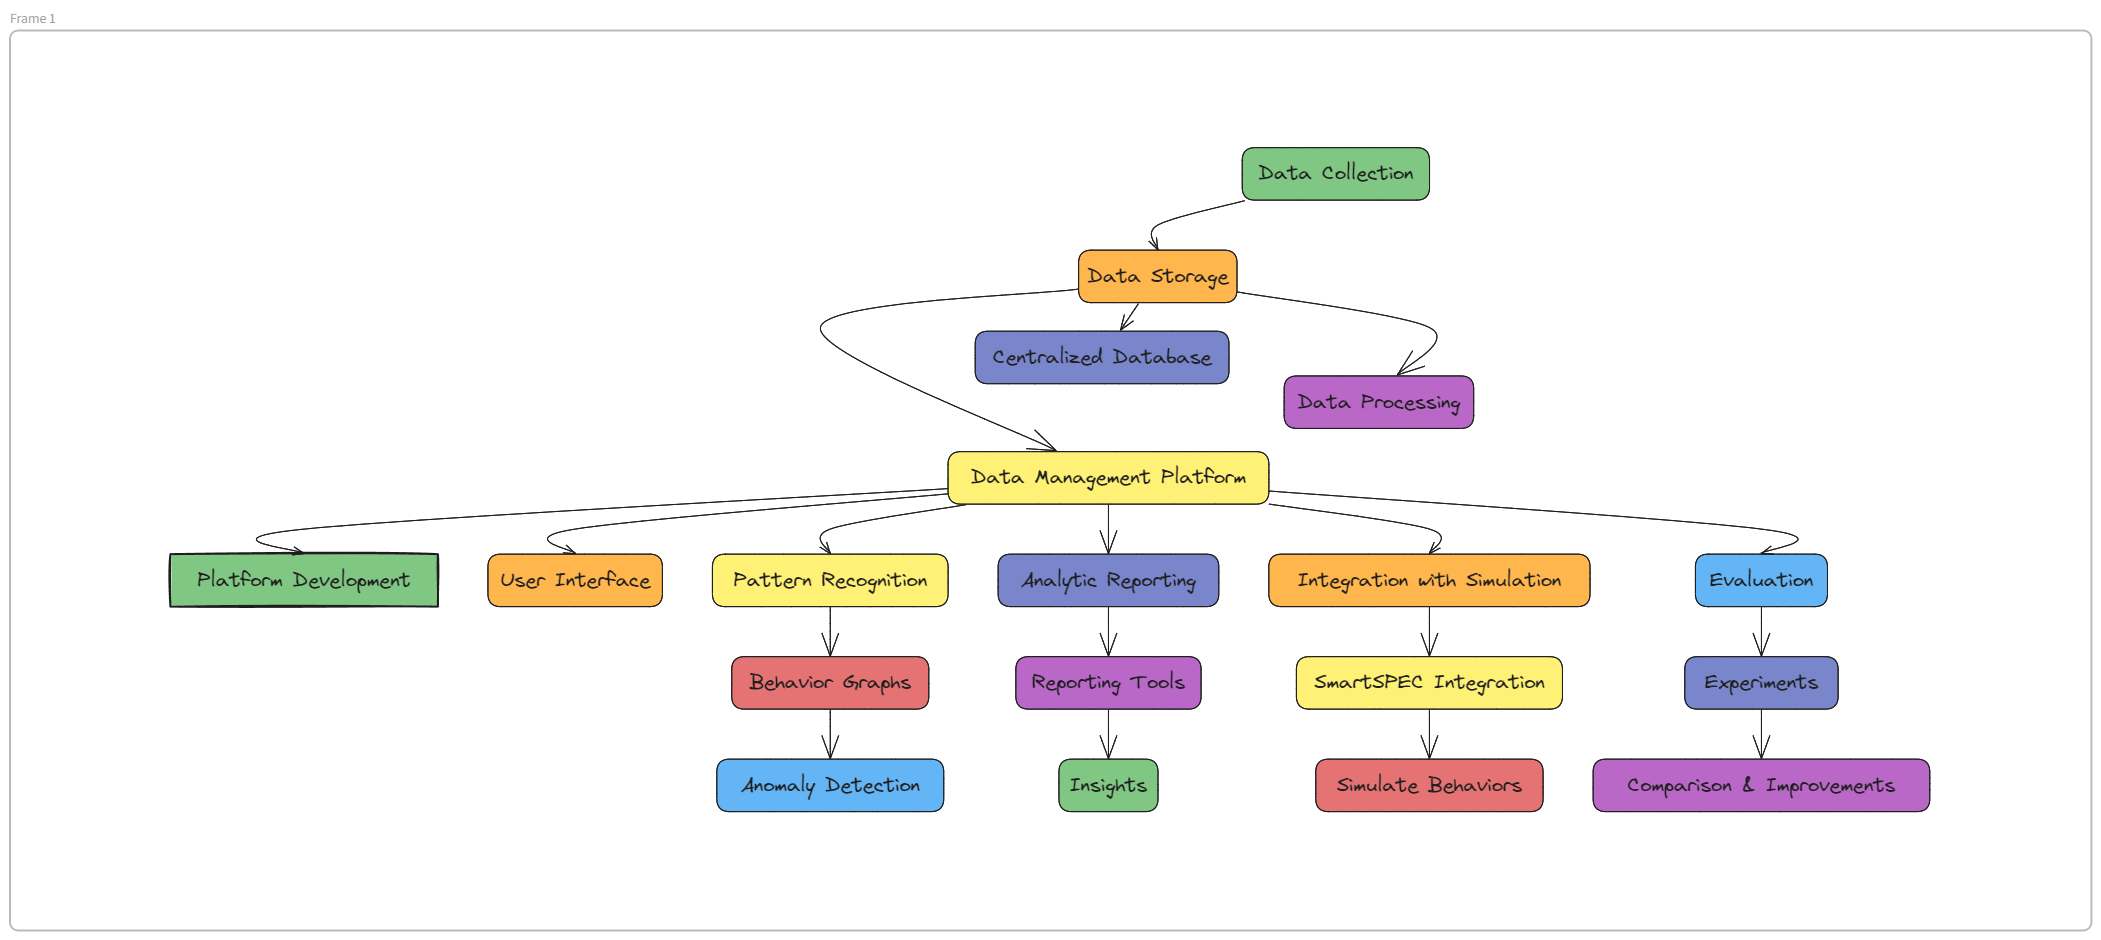
\includegraphics[width=\textwidth]{workflow.png}
    \caption{Workflow of the Data-Driven Agricultural Decision Making Platform}
    \label{fig:workflow}
\end{figure}
Initially, we need to collect data periodically using their API and store it in a centralized database at the university. Once we have this centralized data, we have the freedom to work on it.
After that, we need to create a platform and user interface.\\
Using this data, we can perform analytic reporting to derive interesting results such as cow activities, faulty sensors, and real-time cow location (in this case, we need to call the API and can't rely solely on our cron job to collect data). We will also explore the data to uncover further insights and trends.
By extending this, we can identify patterns and behaviors in cows and create behavior graphs.\\
We can also detect anomalies, such as missing cows or different behaviors due to sickness, and notify users through the platform.
Once we have the methods and models, we can extend SmartSPEC with real sensor data and generate simulation data to aid our solution, conduct experiments, and improve it.\\ \\
Why are we doing this?\\
We are doing this mainly because there is currently no application-specific solution available. This platform could be extended for further research and development and adapted for other similar scenarios.\\
\end{document}
